\documentclass[10pt,a4paper]{ctexart}
\usepackage[margin=2cm]{geometry}
\usepackage{graphicx}
\usepackage{float}      % 支持 [H] 浮动体选项
\usepackage{hyperref}
\usepackage{amsmath}    % 提供方程环境
\usepackage{physics}    % 简化向量、微分算子语法
\newcommand{\myspace}[1]{\par\vspace{#1\baselineskip}} %自定义空一行
\usepackage{fancyhdr}
\pagestyle{fancy}
\fancyhf{}  % 清除所有页眉页脚
\fancyfoot[C]{\thepage}  % 在页脚中央设置页码
\renewcommand{\headrulewidth}{0pt}  % 去掉页眉横线
\renewcommand{\footrulewidth}{0pt}  % 去掉页脚横线

\usepackage{hyperref}
\hypersetup{
    colorlinks=true,
    linkcolor=blue,
    filecolor=magenta,      
    urlcolor=cyan,
    pdftitle={Overleaf Example},
    pdfpagemode=FullScreen,
    }

\usepackage{titlesec}

% 重新定义section格式
\titleformat{\section}
  {\normalfont\Large\bfseries}
  {\chinese{section}、}
  {0pt}
  {}

% 给出常用字号的自定义指令
\newcommand{\chuhao}{\fontsize{42pt}{48pt}\selectfont}
\newcommand{\xiaochu}{\fontsize{36pt}{42pt}\selectfont}
\newcommand{\xiaoer}{\fontsize{18pt}{21.6pt}\selectfont}
\newcommand{\sanhao}{\fontsize{16pt}{20pt}\selectfont}
\newcommand{\xiaosan}{\fontsize{15pt}{18pt}\selectfont}
\newcommand{\sihao}{\fontsize{14pt}{18pt}\selectfont}
\newcommand{\xiaosi}{\fontsize{12pt}{16pt}\selectfont}
\newcommand{\wuhao}{\fontsize{10.5pt}{12.6pt}\selectfont}

% 定义中文数字转换
\titleformat{\section}
  {\normalfont\Large\bfseries}
  {\zhnum{section}、}  % 使用\zhnum而不是\chinese
  {0pt}
  {}

% 标题设置
\title{\xiaochu\textbf{物理实验预习报告}}
\author{}
\date{}

\begin{document}

\vspace*{36pt} % 顶部空白

% 居中填写区域
\begin{center}   
    \xiaochu\textbf{物理实验预习报告}
    % 预留空白区域
    \vspace{13pt}
    \vspace{13pt}
    \vspace{13pt}
    \vspace{13pt}
    
    \sanhao\textbf{实验名称：\underline{\makebox[10cm]{ 交流电路功率因数实验、组装整流器}}} \\[10pt]
    \sanhao\textbf{指导教师：\underline{\makebox[10cm]{ 王宗利 }}} \\[30pt]
    
    % 预留空白区域
    \myspace{6}
    
   \sihao\textbf{班级：\underline{\makebox[6cm]{}}} \\[10pt]
    \sihao\textbf{姓名：\underline{\makebox[6cm]{}}} \\[10pt]
    \sihao\textbf{学号：\underline{\makebox[6cm]{}}} \\[30pt]
    
   \sihao\textbf{实验日期: 
   \underline{\makebox[0.8cm]{2025}}  年 
   \underline{\makebox[0.4cm]{12}}月
   \underline{\makebox[0.4cm]{10}}日  
   星期\underline{\makebox[0.6cm]{三}}上午}
    
    \vspace{18pt}
    \sihao 浙江大学物理实验教学中心
    
\end{center}

\newpage

    \section{实验综述}
    
    \xiaosi （自述实验现象、实验原理和实验方法，不超过300字，5分）

    1.交流电路功率因数实验
    交流电路中负载可以分为感性负载、容性负载和阻性负载。不同负载类型电压和电流相位差不同，阻性负载没有相位差，容性负载电流超前电压90°，
    感性负载电压超前电流90°。因此交流电功率$P=UI \cos(\phi)$，其中$\cos(\phi)$为功率因数。
     \begin{figure}[H]
        \centering
        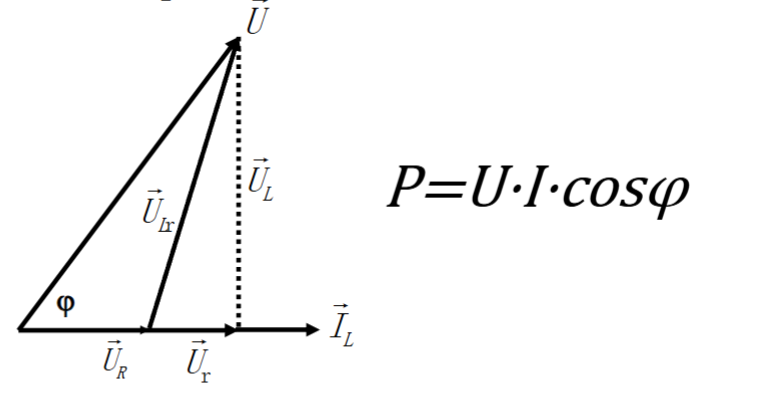
\includegraphics[width=0.6\textwidth]{figure/preview_2.png}
        \caption{功率因数示意图}
        \label{fig:power_factor}
    \end{figure}
    通过在感性负载两端并联电容可以减小$\phi$，提高功率因数。
    \begin{figure}[H]
        \centering
        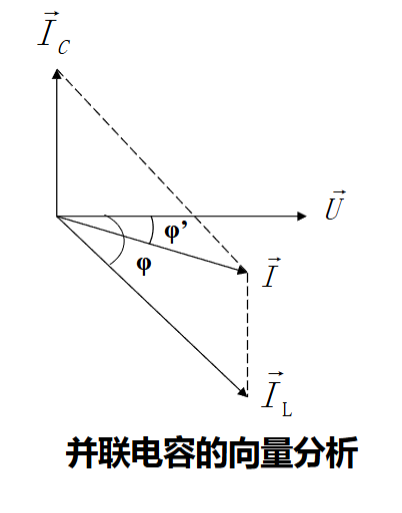
\includegraphics[width=0.6\textwidth]{figure/preview_1.png}
        \caption{并联电容可以提高功率因数示意图}
        \label{fig:power_factor_capacitor}
    \end{figure}
    实验通过改变并联电容大小，测量电流、电压和功率，计算功率因数，拟合功率因数和电容的关系，寻找最佳电容值使功率因数最大。

    实验中使用日光灯作为感性负载。

    2.组装整流器

二极管具有单向导电性，以此为基本原理可以构建整流电路。不同的连接方式可以实现半波整流和全波整流。

    实验中通过组装二极管、电阻、电容等元件，组装成半波和全波整流电路，测量输出电压波形以及平均值、有效值，分析整流效果。

    电容和电感有充放电特性，可以构建滤波电路。实验中通过不使用滤波器和使用不同电容值的滤波器，测量输出波形，分析滤波效果。
    实际生活中整流电路和滤波电路更复杂。也不止包含整流电路和滤波电路，还包含稳压电路等，以满足不同电子设备对电源的要求。
    \begin{figure}[H]
        \centering
        
\includegraphics[width=0.6\textwidth]{figure/circuit.png}
        \caption{电路示意图}
        \label{fig:rectifier_filter}    
    \end{figure}
\myspace{2}
    
    \section{实验重点}
    
    \xiaosi（简述本实验的学习重点，不超过100字，3分）

(1)理解交流电功率因数的概念及其对电路性能的影响。

(2)掌握通过并联电容提高功率因数的方法及其原理。

(3)理解二极管的单向导电特性及其在整流电路中的应用。

(4)掌握组装半波和全波整流电路的方法及滤波电路的基本原理。
    \myspace{2}
    
    \section{实验难点}

    \xiaosi（简述本实验的实现难点，不超过100字，2分）

(1)准确测量交流电路中的电压、电流和功率，计算功率因数。

(2)正确选择并联电容值以优化功率因数。

(3)熟练组装整流电路，确保电路连接正确无误。

(4)分析整流和滤波效果，理解不同滤波器参数对输出波形的影响。
\myspace{2}


\newpage

\sihao\textbf{注意事项：}
\xiaosi
\begin{enumerate}
    \item 用PDF格式上传“预习报告”，文件名：学生姓名+学号+实验名称+周次。
    \item “预习报告”必须递交在“学在浙大”的本课程的对应实验项目的“作业”模块内。
    \item “预习报告”还须拷贝到“实验报告”中（便以教师批改）。
    \item 大学物理实验”课程选做实验使用本“预习报告”；必做实验无须写预习报告，前往“学在浙大”完成预习测试即可。
\end{enumerate}

\vspace{1cm}
\xiaosi\centering \textbf{浙江大学物理实验教学中心制}

\end{document}
